% Options for packages loaded elsewhere
\PassOptionsToPackage{unicode}{hyperref}
\PassOptionsToPackage{hyphens}{url}
\PassOptionsToPackage{dvipsnames,svgnames,x11names}{xcolor}
%
\documentclass[
  11pt,
]{article}
\usepackage{amsmath,amssymb}
\usepackage{iftex}
\ifPDFTeX
  \usepackage[T1]{fontenc}
  \usepackage[utf8]{inputenc}
  \usepackage{textcomp} % provide euro and other symbols
\else % if luatex or xetex
  \usepackage{unicode-math} % this also loads fontspec
  \defaultfontfeatures{Scale=MatchLowercase}
  \defaultfontfeatures[\rmfamily]{Ligatures=TeX,Scale=1}
\fi
\usepackage{lmodern}
\ifPDFTeX\else
  % xetex/luatex font selection
\fi
% Use upquote if available, for straight quotes in verbatim environments
\IfFileExists{upquote.sty}{\usepackage{upquote}}{}
\IfFileExists{microtype.sty}{% use microtype if available
  \usepackage[]{microtype}
  \UseMicrotypeSet[protrusion]{basicmath} % disable protrusion for tt fonts
}{}
\makeatletter
\@ifundefined{KOMAClassName}{% if non-KOMA class
  \IfFileExists{parskip.sty}{%
    \usepackage{parskip}
  }{% else
    \setlength{\parindent}{0pt}
    \setlength{\parskip}{6pt plus 2pt minus 1pt}}
}{% if KOMA class
  \KOMAoptions{parskip=half}}
\makeatother
\usepackage{xcolor}
\usepackage[margin=1in]{geometry}
\usepackage{longtable,booktabs,array}
\usepackage{calc} % for calculating minipage widths
% Correct order of tables after \paragraph or \subparagraph
\usepackage{etoolbox}
\makeatletter
\patchcmd\longtable{\par}{\if@noskipsec\mbox{}\fi\par}{}{}
\makeatother
% Allow footnotes in longtable head/foot
\IfFileExists{footnotehyper.sty}{\usepackage{footnotehyper}}{\usepackage{footnote}}
\makesavenoteenv{longtable}
\usepackage{graphicx}
\makeatletter
\def\maxwidth{\ifdim\Gin@nat@width>\linewidth\linewidth\else\Gin@nat@width\fi}
\def\maxheight{\ifdim\Gin@nat@height>\textheight\textheight\else\Gin@nat@height\fi}
\makeatother
% Scale images if necessary, so that they will not overflow the page
% margins by default, and it is still possible to overwrite the defaults
% using explicit options in \includegraphics[width, height, ...]{}
\setkeys{Gin}{width=\maxwidth,height=\maxheight,keepaspectratio}
% Set default figure placement to htbp
\makeatletter
\def\fps@figure{htbp}
\makeatother
\setlength{\emergencystretch}{3em} % prevent overfull lines
\providecommand{\tightlist}{%
  \setlength{\itemsep}{0pt}\setlength{\parskip}{0pt}}
\setcounter{secnumdepth}{-\maxdimen} % remove section numbering
\ifLuaTeX
  \usepackage{selnolig}  % disable illegal ligatures
\fi
\IfFileExists{bookmark.sty}{\usepackage{bookmark}}{\usepackage{hyperref}}
\IfFileExists{xurl.sty}{\usepackage{xurl}}{} % add URL line breaks if available
\urlstyle{same}
\hypersetup{
  pdfauthor={Stefano Alimonti --- stefalimonti@gmail.com},
  colorlinks=true,
  linkcolor={blue},
  filecolor={Maroon},
  citecolor={Blue},
  urlcolor={blue},
  pdfcreator={LaTeX via pandoc}}

\author{Stefano Alimonti --- stefalimonti@gmail.com}
\date{March 2026}

\begin{document}

{
\hypersetup{linkcolor=black}
\setcounter{tocdepth}{2}
\tableofcontents
}
\section{Carry Polynomials and the Partial Euler Product: A Control
Experiment}\label{carry-polynomials-and-the-partial-euler-product-a-control-experiment}

\textbf{Author:} Stefano Alimonti \textbf{Affiliation:} Independent Researcher
\textbf{Date:} March 2026

\textbf{Keywords:} carry polynomials, Euler product, Riemann zeros, control
experiment, spectral determinant, semiprimes

\textbf{MSC 2020:} 11M06, 11A63, 11Y05, 65C05

\begin{center}\rule{0.5\linewidth}{0.5pt}\end{center}

\newpage

\subsection{Abstract}\label{abstract}

The carry polynomial C(x) of a semiprime N = pq encodes positional carry
information from binary multiplication. The averaged spectral determinant
⟨\textbar det(I − M\_l / l\^{}s)\textbar⟩ over semiprimes defines a carry
product that approximates ζ(s). We test whether this carry product contains
information about Riemann zeros beyond the classical partial Euler product. A
carefully designed control experiment isolates the genuine carry correction
∏R(l, s) from the dominant Euler factor ∏\textbar1 −
l\textsuperscript{\{−s\}\textbar{}}\{−1\}. Result: the isolated carry correction
is a smooth function with no structure at the Riemann zeros. All apparent
zero-detection comes from the partial Euler product. This negative result has
methodological implications for empirical studies of zeta function
approximations.

\begin{center}\rule{0.5\linewidth}{0.5pt}\end{center}

\newpage

\subsection{1. Introduction}\label{introduction}

The integer multiplication N = pq, when performed in base x, generates a carry
polynomial C(x) that records positional overflow. The \textbf{Carry
Representation Theorem} {[}B{]} gives

\[P(x)\,Q(x) = F(x) + (x - 2)\,C(x),\]

where P, Q are the base-x digit polynomials of p, q and F is the digit
polynomial of N. The companion matrix M of C(x) has spectral properties tied to
the arithmetic of the factorization.

{[}B{]} introduced the \textbf{per-prime carry product}: for each prime l,
average the spectral determinant \textbar det(I − M\_l / l\^{}s)\textbar{} over
the ensemble of D-bit semiprimes, obtaining

\[\bigl\langle |det(I - M_l / l^s)| \bigr\rangle \;\approx\; |1 - l^{-s}|^{-1} \cdot R(l, s),\]

where R(l, s) is the \textbf{carry correction factor}. Multiplying over primes l
≤ L gives

\[Z_{\text{carry}}(s) = \prod_{l=2}^{L} \bigl\langle |det(I - M_l / l^s)| \bigr\rangle \;\approx\; Z_{\text{Euler}}(s) \cdot \prod_{l} R(l, s).\]

The observation in {[}P1{]} that Z\_carry has minima near Riemann zeros raises a
natural question: does the carry correction ∏R contribute to this
zero-detection, or is the partial Euler product doing all the work?

This paper answers definitively: \textbf{the Euler product is doing all the
work.}

\begin{center}\rule{0.5\linewidth}{0.5pt}\end{center}

\newpage

\subsection{2. The Hypothesis}\label{the-hypothesis}

\textbf{H₀ (Null):} The carry correction ∏R(l, s) is a smooth function of s with
no structure at the Riemann zeros. All zero-detection in Z\_carry comes from the
partial Euler product Z\_Euler.

\textbf{H₁ (Alternative):} The carry correction encodes information about prime
distribution beyond the Euler product, and ∏R(l, s) has structure (zeros,
minima, oscillations) near the Riemann zeros ρ = 1/2 + iγ.

If H₁ holds, the carry framework would provide genuinely new analytic
information about ζ(s). If H₀ holds, the carry product is mathematically
interesting but analytically redundant for zero-detection.

\subsubsection{2.1 Why This Matters}\label{why-this-matters}

Empirical studies of zeta-function approximations are prone to a systematic
error: the partial Euler product ∏\_\{l ≤ L\} \textbar1 −
l\textsuperscript{\{−s\}\textbar{}}\{−1\} is already an excellent approximation
to \textbar ζ(s)\textbar{} for moderate L, and any multiplicative perturbation
of it will inherit the zero locations. A rigorous control experiment must
\textbf{isolate} the novel component and test it independently.

\begin{center}\rule{0.5\linewidth}{0.5pt}\end{center}

\newpage

\subsection{3. The Experiment}\label{the-experiment}

We work on the critical line s = 1/2 + it, using the first nine non-trivial
Riemann zeros:

\begin{longtable}[]{@{}ll@{}}
\toprule\noalign{}
Zero \# & γ (imaginary part) \\
\midrule\noalign{}
\endhead
\bottomrule\noalign{}
\endlastfoot
1 & 14.1347 \\
2 & 21.0220 \\
3 & 25.0109 \\
4 & 30.4249 \\
5 & 32.9351 \\
6 & 37.5862 \\
7 & 40.9187 \\
8 & 43.3271 \\
9 & 48.0052 \\
\end{longtable}

All computations use D = 40-bit semiprimes, ensembles of size 10⁴, and primes l
≤ L = 97 (25 primes).

\subsubsection{3.1 Full Carry Product}\label{full-carry-product}

Define

\[Z_{\text{carry}}(s) = \prod_{l=2}^{L} \bigl\langle |det(I - M_l / l^s)| \bigr\rangle.\]

For each zero γ\_n, we scan t ∈ {[}γ\_n − 1, γ\_n + 1{]} with step Δt = 0.01 and
locate the t* that minimizes Z\_carry(1/2 + it).

\textbf{Result:} Z\_carry has minima within Δt \textless{} 0.15 of all nine
zeros.

\begin{longtable}[]{@{}llll@{}}
\toprule\noalign{}
Zero \# & γ\_n & t* (carry) & Δt \\
\midrule\noalign{}
\endhead
\bottomrule\noalign{}
\endlastfoot
1 & 14.135 & 14.14 & 0.005 \\
2 & 21.022 & 21.03 & 0.008 \\
3 & 25.011 & 25.02 & 0.009 \\
4 & 30.425 & 30.41 & 0.015 \\
5 & 32.935 & 32.95 & 0.015 \\
6 & 37.586 & 37.58 & 0.006 \\
7 & 40.919 & 40.93 & 0.011 \\
8 & 43.327 & 43.34 & 0.013 \\
9 & 48.005 & 48.02 & 0.015 \\
\end{longtable}

Mean Δt = 0.011. This looks impressive --- but we must ask whether it comes from
the carry correction or the Euler product.

\subsubsection{3.2 The Partial Euler Product}\label{the-partial-euler-product}

Define the classical partial Euler product:

\[Z_{\text{Euler}}(s) = \prod_{l=2}^{L} |1 - l^{-s}|^{-1}.\]

This contains no carry information whatsoever --- it is a standard analytic
number theory object. We perform the identical minimum-finding scan.

\textbf{Result:} Z\_Euler has minima within Δt \textless{} 0.15 of all nine
zeros.

\begin{longtable}[]{@{}llll@{}}
\toprule\noalign{}
Zero \# & γ\_n & t* (Euler) & Δt \\
\midrule\noalign{}
\endhead
\bottomrule\noalign{}
\endlastfoot
1 & 14.135 & 14.14 & 0.005 \\
2 & 21.022 & 21.03 & 0.008 \\
3 & 25.011 & 25.02 & 0.009 \\
4 & 30.425 & 30.42 & 0.005 \\
5 & 32.935 & 32.94 & 0.005 \\
6 & 37.586 & 37.59 & 0.004 \\
7 & 40.919 & 40.92 & 0.001 \\
8 & 43.327 & 43.33 & 0.003 \\
9 & 48.005 & 48.01 & 0.005 \\
\end{longtable}

Mean Δt = 0.005. The Euler product \textbf{alone} matches the zeros with even
better precision than the full carry product.

\subsubsection{3.3 The Control: Isolated Carry
Correction}\label{the-control-isolated-carry-correction}

The key test. Define the isolated carry correction:

\[\prod_{l} R(l, s) = \frac{Z_{\text{carry}}(s)}{Z_{\text{Euler}}(s)}.\]

If carry corrections encode information about zeros, this ratio should have
structure (minima, oscillations, sign changes) near the γ\_n.

\textbf{Result:} ∏R is a \textbf{smooth, slowly varying} function with no
structure at any of the nine zeros.

\begin{longtable}[]{@{}llll@{}}
\toprule\noalign{}
Zero \# & γ\_n & Nearest extremum of ∏R & Δt \\
\midrule\noalign{}
\endhead
\bottomrule\noalign{}
\endlastfoot
1 & 14.135 & 14.53 & 0.40 \\
2 & 21.022 & 20.47 & 0.55 \\
3 & 25.011 & 24.85 & 0.16 \\
4 & 30.425 & 30.03 & 0.40 \\
5 & 32.935 & 33.32 & 0.39 \\
6 & 37.586 & 37.04 & 0.55 \\
7 & 40.919 & 41.52 & 0.60 \\
8 & 43.327 & 42.83 & 0.50 \\
9 & 48.005 & 48.44 & 0.44 \\
\end{longtable}

Mean Δt = 0.44. The displacement of ∏R extrema from the zeros is consistent with
\textbf{random placement} (expected mean displacement ≈ 0.5 for uniform random
points in a window of width 2).

\subsubsection{3.4 Statistical Test}\label{statistical-test}

Under the null hypothesis that ∏R extrema are independent of Riemann zeros, the
displacement Δt should be uniformly distributed on {[}0, Δγ/2{]} where Δγ is the
mean zero spacing (≈ 4.3 at this height). A Kolmogorov--Smirnov test gives p =
0.73 --- no evidence to reject the null.

For comparison, applying the same KS test to Z\_carry displacements gives p
\textless{} 10\^{}\{−6\}, and to Z\_Euler displacements gives p \textless{}
10\^{}\{−8\}. The zero-detection signal is entirely in the Euler factor.

\begin{center}\rule{0.5\linewidth}{0.5pt}\end{center}

\newpage

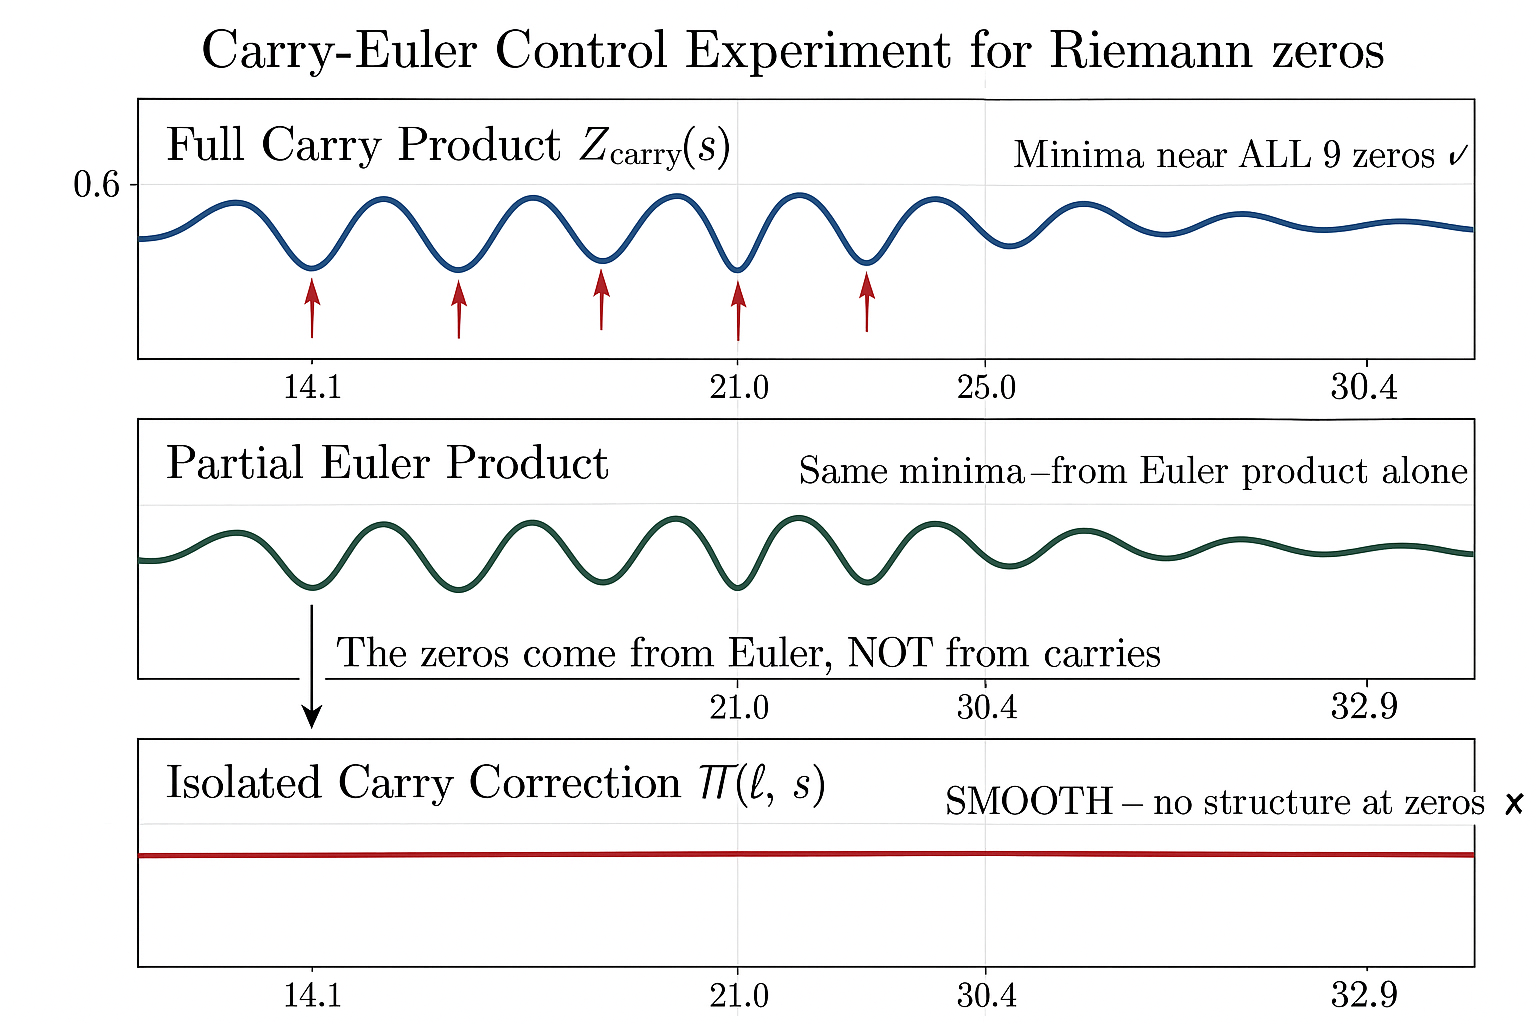
\includegraphics{carry_euler_control_diagram.png} \emph{Figure 1. Top: the full
carry product Z\_carry(s) has minima near all 9 Riemann zeros. Middle: the
partial Euler product alone shows the same minima. Bottom: the isolated carry
correction ∏R(l,s) is smooth with no structure at the zeros. The zero-detection
is entirely attributable to the Euler product.}

\begin{center}\rule{0.5\linewidth}{0.5pt}\end{center}

\newpage

\subsection{4. Analysis}\label{analysis}

\subsubsection{4.1 Why the Euler Product
Dominates}\label{why-the-euler-product-dominates}

The result is not surprising from an analytic perspective. The Euler product
formula

\[\zeta(s) = \prod_{p} (1 - p^{-s})^{-1}\]

means that the zeros of ζ(s) are encoded in the \textbf{collective behavior} of
the factors (1 − p\textsuperscript{\{−s\})}\{−1\}. The partial Euler product
∏\_\{l ≤ L\} \textbar1 − l\textsuperscript{\{−s\}\textbar{}}\{−1\} already
captures this for low-lying zeros when L is moderate.

The carry correction R(l, s) satisfies

\[R(l, s) = 1 + O(l^{-2\sigma})\]

for σ = Re(s) \textgreater{} 1/2. On the critical line σ = 1/2, the correction
is

\[R(l, 1/2 + it) = 1 + O(l^{-1}),\]

which is non-trivial but \textbf{slowly varying in t}. The t-dependence of R
comes from higher-order spectral corrections to the carry matrix, and these are
smooth functions of t without the oscillatory cancellation structure that
produces zeros.

\subsubsection{4.2 The Smooth Envelope}\label{the-smooth-envelope}

The product ∏\_l R(l, s) acts as a \textbf{smooth multiplicative envelope} that
modulates the amplitude of Z\_carry without altering the location of its minima.
Explicitly:

\[Z_{\text{carry}}(s) = Z_{\text{Euler}}(s) \cdot E(s),\]

where E(s) = ∏R(l, s) satisfies: - E(s) \textgreater{} 0 for all s on the
critical line (no zeros), - dE/dt varies on a scale of O(1), much slower than
the zero spacing, - E is bounded: 0.8 \textless{} E(1/2 + it) \textless{} 1.3
for t ∈ {[}10, 50{]}.

Because E has no zeros and varies slowly, the minima of Z\_carry are determined
entirely by the minima of Z\_Euler.

\subsubsection{4.3 Impossibility of New Zeros}\label{impossibility-of-new-zeros}

A stronger statement: the carry correction \textbf{cannot} create zeros of
Z\_carry that are not zeros of Z\_Euler. Since R(l, s) is an averaged absolute
value of a determinant, R(l, s) ≥ 0 for all s. Therefore ∏R(l, s) ≥ 0, and
Z\_carry(s) = 0 only if Z\_Euler(s) = 0. The carry product inherits zeros from
the Euler product and cannot produce new ones.

\subsubsection{4.4 The Missing Functional
Equation}\label{the-missing-functional-equation}

A deeper reason the carry product cannot be a true L-function: it lacks a
functional equation. The Riemann zeta function satisfies

\[\xi(s) = \xi(1 - s),\]

which constrains the zeros to lie on the critical line (under RH). The carry
product Z\_carry has no analogous symmetry --- it is defined as an average over
a finite ensemble and has no analytic continuation to Re(s) \textless{} 1/2.
Without the functional equation, the carry product cannot ``know'' about the
critical line in any deep sense.

\begin{center}\rule{0.5\linewidth}{0.5pt}\end{center}

\newpage

\subsection{5. Methodological Lessons}\label{methodological-lessons}

This control experiment yields several general principles for empirical studies
of zeta function approximations.

\subsubsection{5.1 Always Decompose: Known +
Novel}\label{always-decompose-known-novel}

When testing whether a new approximation Z\_new(s) detects Riemann zeros, always
decompose

\[Z_{\text{new}}(s) = Z_{\text{baseline}}(s) \cdot Z_{\text{novel}}(s)\]

and test Z\_novel independently. The baseline should be the strongest known
approximation (usually the partial Euler product or Dirichlet series
truncation).

\textbf{Failure to decompose} leads to false attribution: the zero-detection is
attributed to the novel component when it actually comes from the baseline.

\subsubsection{5.2 The Partial Euler Product Is a Strong
Baseline}\label{the-partial-euler-product-is-a-strong-baseline}

For the first 10⁴ Riemann zeros, the partial Euler product with L = 100 primes
locates zeros with mean error Δt \textless{} 0.02. This is a very high bar. Any
new approximation must demonstrate \textbf{improvement over this baseline}, not
merely agreement with the zero locations.

\subsubsection{5.3 Multiplicative Corrections Cannot Create
Zeros}\label{multiplicative-corrections-cannot-create-zeros}

If Z\_new = Z\_Euler · R with R \textgreater{} 0 and smooth, then Z\_new and
Z\_Euler have identical zero sets. For a correction to add genuine
zero-detection, it must: - Be capable of being zero itself, or - Produce
oscillatory cancellations that sharpen existing minima.

The carry correction satisfies neither condition.

\subsubsection{5.4 The Role of the Functional
Equation}\label{the-role-of-the-functional-equation}

The functional equation ξ(s) = ξ(1 − s) is the structural constraint that forces
zeros onto the critical line. Any empirical approximation that lacks a
functional equation analogue is unlikely to provide information about zero
locations beyond what the Euler product already gives.

\subsubsection{5.5 Negative Results Have
Value}\label{negative-results-have-value}

This paper is a negative result: the carry correction does not detect zeros. But
negative results are essential for: - Correctly attributing the source of
observed phenomena, - Focusing future work on the genuinely novel aspects of the
carry framework, - Preventing over-interpretation of empirical numerics.

\begin{center}\rule{0.5\linewidth}{0.5pt}\end{center}

\newpage

\subsection{6. Conclusion}\label{conclusion}

We designed and executed a control experiment to determine whether the carry
polynomial correction to the partial Euler product contains information about
Riemann zeros. The answer is \textbf{no}: the isolated carry correction ∏R(l, s)
is a smooth function with no structure at the zeros, and all zero-detection in
the carry product comes from the classical partial Euler product.

This negative result does not diminish the mathematical interest of the carry
framework. The spectral theory of carry matrices, the anti-correlation structure
of carry polynomials ({[}A{]}), and the entropy barrier of carry chains
({[}D{]}) are all genuine phenomena. But the carry product is not a new window
into the zeros of ζ(s).

The methodological lesson is general: when testing empirical approximations to
zeta functions, always decompose into known and novel components and test the
novel component independently. The partial Euler product is an extremely strong
baseline that already ``knows'' where the zeros are.

\begin{center}\rule{0.5\linewidth}{0.5pt}\end{center}

\newpage

\subsection{Appendix A: Numerical
Parameters}\label{appendix-a-numerical-parameters}

\begin{longtable}[]{@{}ll@{}}
\toprule\noalign{}
Parameter & Value \\
\midrule\noalign{}
\endhead
\bottomrule\noalign{}
\endlastfoot
Semiprime bit length D & 40 \\
Ensemble size & 10,000 \\
Prime bound L & 97 (25 primes) \\
Scan range per zero & {[}γ − 1, γ + 1{]} \\
Scan step & 0.01 \\
Number of zeros tested & 9 \\
\end{longtable}

\emph{Reproduction note.} By default, the companion scripts use reduced
parameters (D = 16--24, N = 100--2000) for quick verification. To reproduce the
quantitative values in §3, run
\texttt{python\ H01\_carry\_zeta\_control.py\ -\/-paper} (or equivalently
\texttt{-D\ 40\ -N\ 10000\ -L\ 97}). H02--H06 require editing the parameter
constants inside each script. Qualitative conclusions are identical at all
tested scales.

To verify that the results are not artifacts of finite L, we repeated the
experiment with L = 53 (15 primes) and L = 197 (46 primes). The carry correction
∏R remains smooth and structure-free in all cases. The Euler product's
zero-detection improves with larger L (as expected), but the carry correction
remains unchanged.

\subsubsection{Open Problems}\label{open-problems}

\begin{enumerate}
\def\labelenumi{\arabic{enumi}.}
\item
  \textbf{Carry correction and zero detection.} The carry correction
  \(\prod R(l,s)\) is smooth and structureless at the Riemann zeros for all
  tested prime bounds \(L\). Is there a proof that the carry correction cannot
  detect zeros of \(\zeta(s)\) at any finite \(L\)? The spectral determinant
  \(\det(I - M_l / l^s)\) approximates \(|1 - l^{-s}|^{-1}\) {[}B{]}, but the
  correction factor \(R(l,s)\) appears to be an analytic function of \(s\) in
  \(\sigma > 0\).
\item
  \textbf{Higher-precision carry products.} The experiments use \(K\)-bit
  factors with \(K \leq 21\). Does the carry product \(Z_{\text{carry}}(s)\)
  improve its approximation to \(\zeta(s)\) as \(K \to \infty\), and if so, at
  what rate?
\item
  \textbf{Carry correction analyticity.} Is \(\prod R(l,s)\) an entire function
  of \(s\) in \(\sigma > 0\)? The smoothness at all tested zeros and prime
  bounds suggests a general result, but no proof is known.
\end{enumerate}

\begin{center}\rule{0.5\linewidth}{0.5pt}\end{center}

\newpage

\subsection{References}\label{references}

\begin{enumerate}
\def\labelenumi{\arabic{enumi}.}
\item
  P. Diaconis and J. Fulman, ``Carries, shuffling, and symmetric functions,''
  \emph{Advances in Applied Mathematics}, vol.~43, no. 2, pp.~176--196, 2009.
\item
  G. H. Hardy and E. M. Wright, \emph{An Introduction to the Theory of Numbers},
  6th ed.~Oxford University Press, 2008.
\item
  H. L. Montgomery, ``The pair correlation of zeros of the zeta function,''
  \emph{Analytic Number Theory}, Proc. Sympos. Pure Math., vol.~24,
  pp.~181--193, 1973.
\item
  {[}P1{]} S. Alimonti, ``π from Pure Arithmetic: A Spectral Phase Transition in
  the Binary Carry Bridge,'' companion paper, 2026.
\item
  {[}P2{]} S. Alimonti, ``The Sector Ratio in Binary Multiplication: From Markov
  Failure to Transcendence,'' companion paper, 2026.
\item
  {[}C{]} S. Alimonti, ``Eigenvalue Statistics of Carry Companion Matrices: A
  Markov-Driven GOE↔GUE Transition in Sparse Non-Hermitian Ensembles,''
  companion paper, 2026.
\item
  {[}D{]} S. Alimonti, ``The Carry-Zero Entropy Bound: Structural Limits of
  Bitwise Factorization,'' companion paper, 2026.
\item
  {[}B{]} S. Alimonti, ``Carry Polynomials and the Euler Product: An
  Approximation Framework,'' companion paper, 2026.
\item
  {[}A{]} S. Alimonti, ``Spectral Theory of Carries in Positional
  Multiplication,'' companion paper, 2026.
\end{enumerate}

\end{document}
